\section{Yusuf Jordan El Anwar - 1184026}
\subsection{Teori}
\begin{enumerate}

	\item Definisi Kecerdasan Buatan
	\hfill\break
	Kecerdasan buatan atau artificial intelligence (AI) adalah sebuah teknologi buatan manusia yang di modelkan ke dalam sebuah mesin dan mesin di tersebut di program supaya dapat berpikir seperti manusia sehingga dapat bekerja layaknya manusia dan berpikir seperti manusia sehingga dapat memudahkan pekerjaan manusia.

    AI ini merupakan sebuah mesin dan tidak memiliki kecerdasan sehingga untuk itu kita perlu menambahkan data dan pengalaman kepada mesin tersebut supaya mesin tersebut dapat memiliki kecerdasan. Point penting didalam ai adalah learning, reasoning, dan self correcting.
	\item Sejarah dan Perkembangan
	\hfill\break
    AI tersusun dari 2 kata yaitu artificial intelligence. Intelligence sendiri berasal dari kata Yunani “intelligo” yang memiliki arti “saya paham”. Dan intelligence memiliki arti dasar kemampuan untuk memahami kemudian pemahaman tersebut di lakukan.
    Sejarah kecerdasan buatan sudah ada pada zaman kuno namun dikenal sebagai cerita tentang mahkluk buatan yang diberkahi oleh para pengrajin. Sehingga akhirnya sebuah karya memuncak saat penemuan komputer digital yang diprogram pada tahun 1940-an.
    Pada tahun 1965 istilah kecerdasan buatan pertama kali di perkenalkan di konferensi darthmouth dan dikembangkan hingga sekarang
    Sekitar akhir tahun 1955, Newell dan Simon mengembangkan program ai pertama yang di namakan The Logic Theorist. Program ini memiliki dampak yang besar dan menjadi batu loncatan penting dalam sejarah perkembangan  AI. Satu tahun setelahnya yaitu pada tahun 1956 John McCarthy guru dari Massacuhetts Institute of Technology dianggap sebagai bapak AI karena menyelenggarakan konferensi “The Dartmouth summer research project on artificial intelligence” untuk menarik para ahli komputer bertemu.  Di Konferensi Dartmouth itu akhirnya mempertemukan cikal bakal para pendiri dalam AI yang akhirnya  meletakkan dasar bagi generasi di masa depan untuk  mengembangkan dan melakukan penelitian pada bidang AI. Sekitar  tahun 1960 hingga 1970 muncul berbagai komunitas yang berdiskusi bagaimana komputer dapat meniru sedetail mungkin pada kemampuan otak manusia sehingga memunculkan isitilah “classical AI”. Mulai tahun 1980, computer semakin mudah diperoleh dengan harga yang lebih murah, sehingga menjadikan berbagai riset di bidang kecerdasan buatan semakin berkembang pesat pada berbagai universitas.
    Perkembangan awal AI ( 1952 - 1969 )
    Perkembangan awal ai di mulai ketika Newell dan Simon membuat sebuah program yang dikenal sebagai General Problem Solver yang dirancang untuk mengembangkan sebuah penyelesaian masalah secara manusiawi yang akhirnya berakhir dengan kesuksesan.
    Di lanjutkan oleh James Slagel pada tahun 1963 yaitu membuat sebuah program untuk menyelesaikan masalah integral tertutup untuk membantu pada bidang matakuliah kalkulus.
    Dan terakhir pembuatan program untuk memberikan analalogi penyelesaian masalah analogi geometris pada tes iq yang di ciptakan oleh Tom Evans.
    Perkembangan Kecerdasan Buatan ( 1966  –  1974 )
    Pada fase ini perkembangan kecerdasan mulai melambat karena beberapa factor. Yaitu : 
    Pertama, Program yang berhasil  hanya diciptakan karena manipulasi program sebelumnya.
    Kedua, Banyak masalah masalah kompleksyang harus di selesaikan kecerdasan buatan.
    Ketiga, Mulai adanya beberapa Batasan pada struktur dasar sehingga menyulitkan untuk menghasilkan perilaku intelligence.
    Sistem berbasis Pengetahuan ( 1969 - 1979 )
     Ed Feingenbaum, Bruce Buchanan dan Joshua Lederberg berhasil membuat sebuah program untuk memecahkan masalah struktur molekul dalam bidang kimia
    Industri Kecerdasan Buatan ( 1980 – 1988 )
    Kecerdasan buatan mulai merambah dunia industry ketika ditemukannya system pakar yang bernama R1 yang dapat mengkonfigurasi system – system pada computer baru.
    Jaringan Syaraf Tiruan ( 1986 – Sekarang )
    Sekelompok periset menemukan algoritma yang di implementasikan pada bidang ilmu computer dan psikologi .  algoritma ini di namakan algoritma belajar propagasi balik.
\begin{itemize}
		\item Supervised dan Unsupervised Learning
		\hfill\break
	Supervised learning adalah metode pendekatan pengelompokan data atau variable yang sudah di targetkan dan mengelompokan data tersebut ke dalam data yang telah ada. Sedangakn Unsupervised learning adalah metode pendekatan yang tidak memliki data sehingga data yang ada harus di pilah menjadi beberapa kategori atau bagian.
		\item Klasifikasi dan Regresi
		\hfill\break
		Klasifikasi adalah sebuah metode pengelompokan data berdasarkan standard yang telah ada. Sedangkan regresi adalah sebuah metode analisis statistik untuk melihat bagaimana pengaruh suatu variable.
		\item Definisi Dataset, Trainig Set dan Testing Set
		\hfill\break
        Dataset adalah objek yang berfungsi untuk mempresentasikan data atau relasi di dalam memori.
        Training set adalah bagian dataset yang dapat membuat memprediksi atau algoritma berdasarkan tujuan masing masing
        Testing Set adalah bagian dari dataset dilakukan tes untuk melihat seberapa akurat dan ketepatan datanya.  
	\end{itemize}
\end{enumerate}
\subsection{Praktek}
\begin{enumerate}
\item Instalasi Library scikit dari Anaconda, mencoba kompilasi dan uji coba ambil contoh kode dan lihat variabel explorer
	\hfill\break
	\begin{figure}[h]
		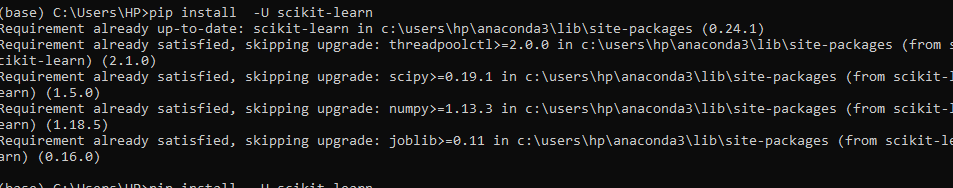
\includegraphics[width=10cm]{figures/1184026/chapter1/Capture.PNG}
		\centering
		\caption{Instalasi Library Scikit Learn}
	\end{figure}
	\begin{figure}[h]
		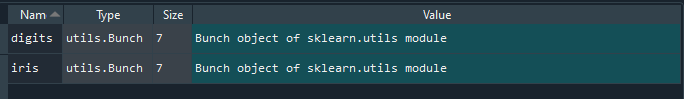
\includegraphics[width=10cm]{figures/1184026/chapter1/variabel eksplore.PNG}
		\centering
		\caption{Isi Variabel Explorer}
	\end{figure}
	\item Uji coba loading an example dataset
	\hfill\break
\lstinputlisting[firstline=1, lastline=4]{src/1184026/chapter1/belajar.py}
\item Uji coba Learning dan predicting
	\hfill\break
	\lstinputlisting[firstline=8, lastline=15]{src/1184026/chapter1/contoh2.py}
\item Uji coba Model Persistence
	\hfill\break
	\lstinputlisting[firstline=8, lastline=32]{src/1184026/chapter1/contoh3.py}
	\item Uji coba Conventions
	\hfill\break
	\lstinputlisting[firstline=8, lastline=19]{src/1184026/chapter1/contoh4.py}
\end{enumerate}
\begin{enumerate}
	\item ScreenShoot Error
	\begin{figure}[h]
		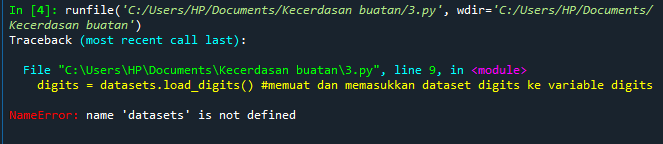
\includegraphics[width=10cm]{figures/1184026/chapter1/eror1.PNG}
		\centering
		\caption{Name Error}
	\end{figure}
	\item Tuliskan Kode Error dan Jenis Error
	\hfill\break
	Name 'datasets' is not defined
\hfill\break
	\item Cara Penangan Error
\hfill\break Tambahkan variabel datasets agar kode program dapat terbaca
	\end{enumerate}
